Mutation testing research dates back to the 70s, and has long aimed to render
mutation testing useful for constructing high quality
test suites and, by extension, software.
Most of this previous
research focuses on computing a mutation score, a measure of adequacy for a
given test suite.  However, this is computationally intensive for realistic
projects, because it requires requires running many tests on many modified
versions of a software system.  Reducing that computational cost is thus a major
thrust of mutation testing research~\cite{jia2011analysis}.

Moreover, although test suite adequacy is certainly a useful thing to measure, the most
important goal of mutation testing\,---\,and indeed its original use
case~\cite{budd1980theoretical}\,---\,is to help \emph{improve} a test suite.  For this
purpose, either a score or a vast list of all unkilled mutants is not useful for practicing engineers.  An
undifferentiated list of unkilled mutants typically contains mostly uninteresting or
redundant mutants, and a much smaller number of actionable mutants that are
maximally useful in guiding test improvement.  Examining all unkilled
mutants is only practical for formal verification efforts or critical
systems with high-powered test suites.

But even in these settings, examining
surviving mutants produced by comprehensive mutation testing campaigns is
time-consuming and unpleasant, as PI Groce and co-authors noted in prior work on
using mutants to drive formal verification and automated
testing~\cite{groce2015verified,groce2018verified,mutKernel}.
%
That work proposes a novel approach to
formal verification and automated testing
combining Karl Popper's falsification-based notion of
scientific discovery~\cite{Popper,popperconjectures} with mutation
testing~\cite{groce2015verified,groce2018verified,mutKernel}.
The heart of the idea is (1) a surviving non-equivalent mutant
\emph{falsifies} the claim that a given
formal verification or test effort captures a full notion of
correctness and (2) refining a
verification or testing effort by repeated efforts at falsification is an
effective method for ensuring the quality of verification and testing
efforts.  The
approach allowed Groce and colleagues to identify of multiple previously unknown faults in
the Linux kernel's
RCU~\cite{MathieuDesnoyers2012URCU,DinakarGuniguntala2008IBMSysJ,McKenney:2013:SDS:2483852.2483867}
module and the {\tt pyfakefs} Python mock file
system~\cite{pyfakefs}, despite the existence of very-high-quality
automated test generation efforts for these
systems~\cite{rcutorture,TSTL}.  This prior work
proposed a number of algorithms and
methods for finding bugs in testing and verification
harnesses.  At a high level, however,
the core concept is simple:  users should examine all unkilled
mutants, and for each mutant either understand why it is
equivalent or uninteresting, or actually construct a way to kill it.  In a sense, this harkens back to the
earliest ideas about mutation testing, but with
much more automated support.

Unfortunately, the
methods proposed were, while useful, limited in applicability.  They simply assumed that the number of unkilled mutants was
small, and focused on solving the problem of helping a developer or
test engineer kill surviving mutants.
In practice, however, human
attention does not scale to analyzing large numbers of
unkilled mutants without further assistance in ``triaging'' them.  The process bears a
resemblance to the problem of manual confirmation of results from a
machine-learning classifier~\cite{OnlyOracle,EndUserMistake}, where even highly-motivated scientific
users are unwilling to examine more than a few tens of
potentially incorrect results~\cite{Segal}.
This prior approach suffers the same problems as other
mutation testing efforts: it provides no way to
scale human efforts to such a needle-in-a-haystack setting.

This project aims to make the falsification-driven approach to verification and testing feasible for larger
projects, and those with lower mutation scores.
Our goal is to enable \emph{Just Enough Mutation Testing}: We propose a mutation
testing framework that identifies and interactively presents a few, very
different, ranked mutants, and then \emph{works with the user} to 
effectively improve the program, the test suite, or both.

Figure \ref{fig:flow} shows the basic outline of a proposed workflow.
%
This framework aims to generate a small, diverse set of
mutants, chiefly characterized by their novelty, to present to the developer or
test engineer.  The framework further works
 \emph{with} the test engineer to improve the SUT or
the underlying tests, and incorporate user feedback into which mutants are
interesting or useful (or not).  This results in a constantly-updated ranking of mutants,
based on actions and feedback from the engineer.

A key insight behind our proposed approach is to view mutant triage as
analogous to the bug triage
(a.k.a.  ``fuzzer
taming'') problem in random testing/fuzzing~\cite{PLDI13,distMut,SemCrash,vantonder-ase18}:  a user wants
to quickly find mutants that indicate the most important ``holes'' in a testing
or verification effort, and act on those most-critical gaps, possibly revealing
faults in the System Under Test (SUT).
An unkilled mutant is, conceptually, very similar to a failing test.
Fuzzers tend to produce very large numbers of failing tests for a much
smaller number of distinct bugs.  Finding the set of distinct bugs,
and identifying important bugs that need to be fixed immediately is
difficult, because the important bugs may be represented by only one
or two failing tests in a set of thousands of failing tests, most of
which are duplicates.
Users do not (usually) care much
about finding the group of all tests failing due to a fault, or the
set of all mutants killable by the same extension to a test suite or
generator, but about seeing \emph{many very different test failures}
or \emph{many
  different unkilled mutants} quickly, to maximize the chance of
discovering the most important faults or holes in a testing effort.
Our approach thus fundamentally seeks to identify a small set of maximally different, maximally interesting mutants to present
to the user.

\begin{wrapfigure}{r}{.5\textwidth}
\centering 
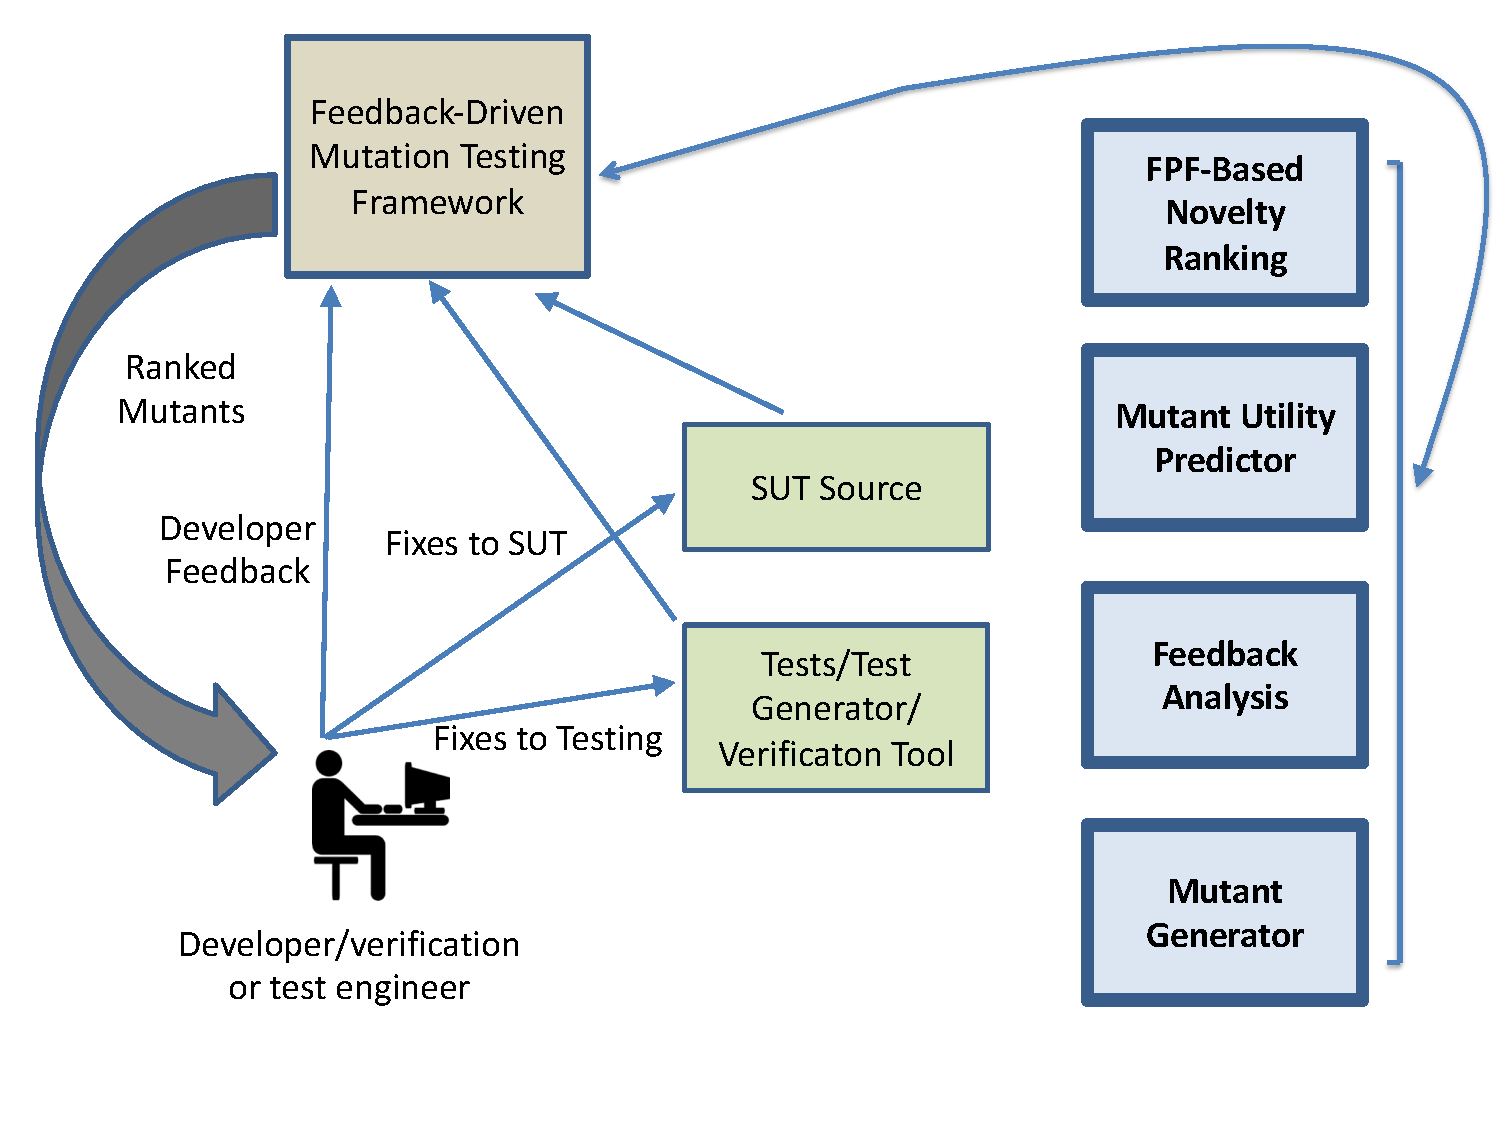
\includegraphics[width=0.5\textwidth]{TestFlow}

\caption{Proposed mutation workflow. }
\label{fig:flow}
\end{wrapfigure}



A second important principle behind our approach is to take advantage of user
feedback in refining the list of interesting mutants and improving the SUT.
A test engineer has valuable insight\,---\,and the final word\,---\,about which
unkilled mutants are uninteresting or equivalent, and which require changes to
the system itself or the test harness.  We propose to explicitly take this
feedback into account, refining the analysis accordingly, as the user improves
their system.  Beyond allowing for more effective mutation analysis,
this new paradigm provides a stopping rule other than patience, time available, or
``every last mutant'':  since mutants are ranked by likely payoff, once a user
has examined several mutants in a row without benefit, or mutants are highly
similar in behavior to other mutants, a user may reasonably stop, knowing that
the low-hanging fruit have probably all been picked.
 It also enables a new way to improve the efficiency of
mutation testing:  even for a very large project, it only has to build and
execute a small set of mutants, because it only runs the test suite on mutants
currently predicted to be of likely interest to the user.

Overall, our approach requires several fundamental research novelties:
\begin{itemize}[labelsep=3pt,leftmargin=12pt]
\item \textbf{Efficient, any-language mutation testing.}
Our goal of user-interactive mutation testing, integrated directly into
the development and test process, requires that mutation generation be
\emph{source-level} and \emph{multi-language}.
Bytecode-level mutation is highly effective for computing
mutation scores~\cite{pittest,HaririLLVM}.  However, developers or test
engineers reason more naturally about a mutant's implications when mutations
are presented in the source language in question.  Moreover, modern mutation
testing frameworks are limited to specific languages, or to IR-defined
ecosystems like LLVM or Java bytecode.  This leaves out popular languages like Python, Ruby, or Go, not
to mention project-specific Domain Specific Languages (DSLs)~\cite{Fow10}.
Meanwhile, the vast majority of
real-world software projects are written in multiple languages~\cite{Ray2014}.
We therefore propose novel mechanisms for \emph{efficient, any language mutation
  testing} based on our novel recent work on language-agnostic declarative
program transformation~\cite{rvt-ppc}.
\item \textbf{Mutant prioritization and selection.}  Our
  proposed framework will present a small, maximally-informative ranked list of
  mutants to the user.
Current mutation testing approaches make
no real effort, with few exceptions~\cite{MutGoogle,FaRM} to prioritize mutants.
Other than (arguably) some efforts to
incorporate dominance results~\cite{MutQuality}, mutation testing approaches
currently offer no way to maximize the novelty of presented
mutants than stratified sampling~\cite{gopinath2017mutation}, which
does not aim at (or achieve) significant semantic novelty.  Thus,
we propose to adapt clustering optimization techniques based on 
novelty~\cite{Gonzalez85} to the problem of mutant selection, informed by a set
of novel diversity metrics for the domain.
\item \textbf{User feedback elicitation and analysis.}
A
user's feedback about the most critical-to-test aspects of the code, or hard
work examining some mutants, has no influence on the kinds of sampling currently
proposed in the mutation testing literature.
Even creating simple clusters of
mutants that are not killed due to the same underlying omission in tests
requires manual effort, with users, e.g., writing a Python script scanning
mutants for certain strings and assuming all mutated code with that string is
part of the same ``equivalence class.''  This is a tedious and error-prone
process, and only even possible once a ``kind'' of unkilled mutant is
discovered, largely by ad hoc scanning of the list of unkilled, uncategorized,
mutants.
We propose ``feedback-driven'' mutation analysis that elicits and incorporates
user input on mutants, tests, and the SUT, supporting a concise, updating list
of mutants to inspect based on expected utility or payoff for the
user.  Feedback also opens up new ways to execute fewer mutants, 
often in parallel with useful user activity.
\end{itemize}

%Because our proposed feedback-driven approach no longer requires small absolute
%numbers of unkilled mutants, it extends the applicability of the approach to
%using manual tests to kill mutants, which was not in scope when extremely high
%kill-rates were required.

\subsection{Problem Statement}

Overall, this project aims to make the use of program mutants practical in
non-research settings, in a way that meets developers' actual needs: to make it
possible for someone creating or enhancing a test suite to (1) use ``just
enough'' mutation testing for their needs, maximizing benefit gained in exchange
for work performed, and to (2) work in any programming language(s) without worrying
about the quality of tool support, using intuitive source-based
mutants and easy customization
%This project also aims to extend the insights of
%Test-Driven-Development (TDD) 
%beyond a paradigm where developers build a series of tests narrowly tailored to
%steps in development, and use Mutation-Driven-Development (MDD) to build
%automated test generators or verification harnesses that handle not only
%anticipated problems imagined during development, but problems not anticipated
%by developers.
In addition to traditional manual testing, this proposal targets
property-driven testing and formal verification, in
order to be practical in the future, when many systems will be so
safety- or mission- critical that even ``good'' manual testing is simply not 
acceptable, by extending Test-Driven-Development (TDD) to become
Mutation-Driven-Development (MDD).


\begin{framed} {\bf Problem:} Develop highly automated methods and tools that
  allow the practical application of mutation testing to real-world software in
  a feedback-driven way, where user and mutation testing framework cooperate to
  improve testing efforts, while minimizing user effort and maximizing the
  ability to quickly find the most important weaknesses of testing or
  verification.
\end{framed}

% \begin{framed}
% {\bf Problem:}  Provide high-quality user-friendly mutation generation methods to be used in a flexible but efficient mutation testing framework that can be applied to any source language, with support for easily adding custom operators or mutating DSLs.
% \end{framed}


\subsection{PI Qualifications}

PI Groce has been a user of, and contributor to, mutation testing tools for many
years.  He combines a long research track record in software testing, including
mutation testing, with actual experience testing critical software systems at
NASA's Jet Propulsion Laboratory.  PI Groce's long-running interest in improving
mutation testing arises from frustration in his efforts to apply mutation to the
Mars Science Laboratory's flight software, in particular to the file
system~\cite{ICSEDiff,CFV08,AMAI}.  This practical orientation informs his
recent work on using mutation testing in a falsification-driven approach to
improving verification and automated testing
efforts~\cite{groce2015verified,groce2018verified,mutKernel}.  PI Groce has
extensive experience in developing mutation tools for new
languages~\cite{le2014mucheck,muupi,regexpMut}, including the first reliable
tools for mutation of Haskell, Python, and Swift, as well as in user-facing
(vs. researcher-oriented) automated software testing
tools~\cite{tstlsttt,DeepState}.  He additionally has expertise in driving
testing of machine learning systems through user
interaction~\cite{EndUserMistake,OnlyOracle}.

PI Le Goues is an expert in applied program analysis, program transformation,
and testing, most relevantly through her pioneering work in automated program
repair (including heuristic~\cite{legouesNFWTSE2012} and
semantic~\cite{s3,Ke15ase} dynamic approaches, and approaches guided by
static analysis~\cite{footpatch}).  She has significant experience
with testing, mutation testing for fault localization and program repair
particularly~\cite{ssbse}, and the challenges of syntactic program
modification and transformation.  In particular, her recent work has developed
novel mechanisms for efficient and expressive language-agnostic syntactic
program transformation~\cite{rvt-ppc}, with applications for, e.g., program
repair~\cite{footpatch}, fuzz test triage~\cite{vantonder-ase18}, and static analysis
customization~\cite{vantonder-tailoring19}.

The PIs provide a detailed work and collaboration plan in the Collaboration Plan
supplementary document.
